\subsection{Component view}
In this section, components are expanded and better analyzed. \\
The main analysis regards the microservices block: 
\begin{figure}[H]
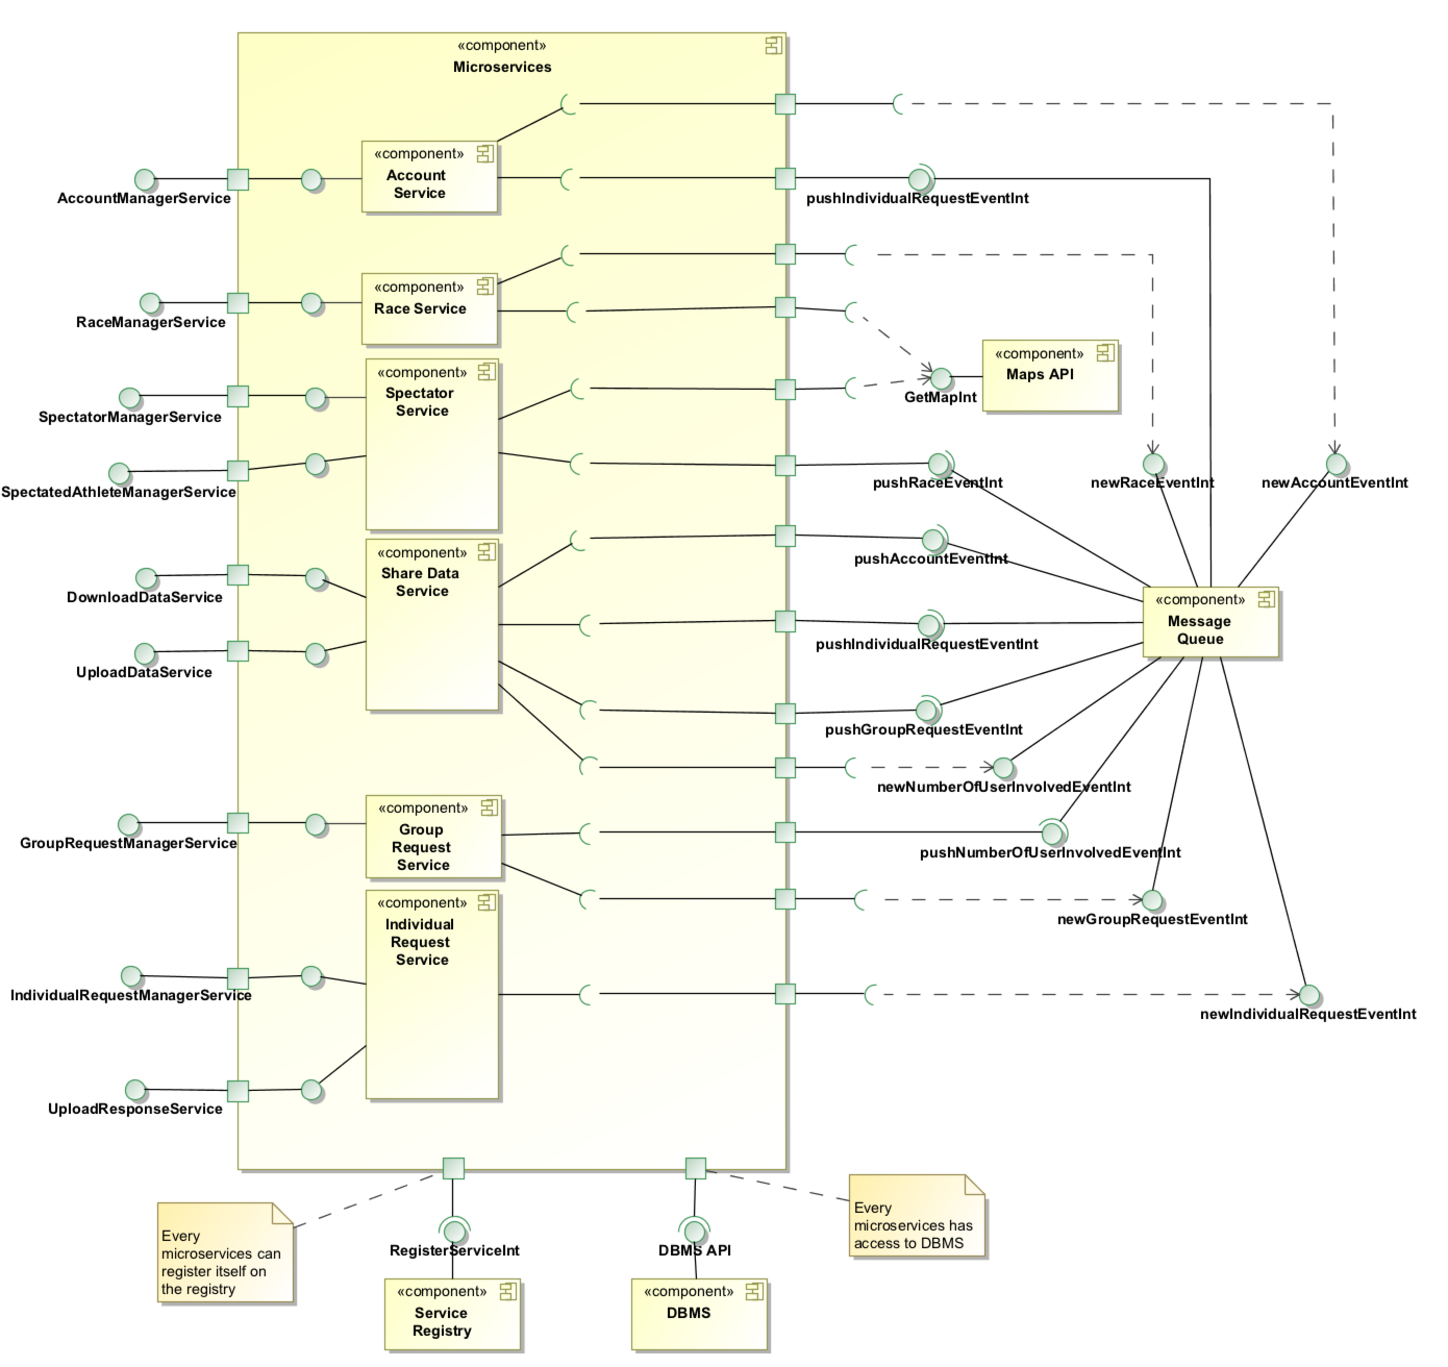
\includegraphics[width=\linewidth]{Images/componentdiagram.pdf}
\caption{ Component diagram }
\label{fig:world2}
\end{figure}
Various service components are present, and they all expose at least an interface that is accessed by the
clients via the API gateway. It follows a brief description of the various services, and a better
specification of what their interfaces provide:
\begin{itemize}
\item The account service provides all the functions related to user sessions, such as login and logout,
and also the registration of clients (both user and third party customer)
\item The race service makes possible for an athlete to enroll in a run; for a third party customer to set
up one, and also close it; and it also enables the possibility of retrieving the available races and their
status (e.g. in course, terminated and so on and so forth). Therefore, it manages the "more static" part
of a race
\item The spectator service regards the dynamic part of a race, such as the fact that user can spectate
the athletes who are running (therefore they can retrieve their positions and the leaderboard). This
service, is also in charge of receiving position data of the participants
\item Share data service is responsible for the monitoring of user health statuses and positions: here a
user will upload his data. Furthermore, third party customer will access the data that they have
previously requested, by means of "DownloadDataService" interface
\item The group request service provides to the third parties the possibility of uploading group requests and see their status 
\item The individual request service enables third party customer to upload individual request and monitor their status, and allows a user to check if there are some requests for him and upload responses 
\end{itemize}

All the microservices have their own data and therefore access DBMS's API, while Maps's API are necessary 
only for race and spectator service, in order to manage and double check position data and feasible paths
\\
The diagram also shows the main communications that take place between components. The following message exchange is needed to completely and
correctly exploit the project functions. More specifically, when a third party is accessing data through the data share service, this access
needs to be verified by one among group request service and individual request service (depending on the type of data that the customer is
trying to obtain). Indeed, the request acceptance and its data, are managed by the two above mentioned components. \\ 
The other important message exchange is between spectator and race services: in particular, data that the spectator service is receiving must
be matched with an active run, and thus a validation process is taking place here. \\